\chapter{Related Work}
\label{chap:relwork}

The area of relational learning in the context of Semantic Web has recently attracted interest from many researchers. The approaches that aim at tackling this problem can be mainly classified into three groups: statistics-based, text-based and logic-based. In this chapter we review Semantic Web and the relevant works from these groups.

\section{Semantic Web}

The Semantic Web~\cite{ref26} is a paradigm that enables computers to interpret the meaning of the data from the Internet. Alternatively, it is defined as ``a web of data that can be processed directly and indirectly by machines".

The World Wide Web Consortium (W3C) defines the Semantic Web and the Resource Description Framework (RDF) as a platform for Linked Data~\cite{ref26}. The W3C proposes other technologies such as SPARQL and OWL for data manipulation. Architecture of the W3C is presented as a stack in Figure~\ref{fig1}~\footnote{\url{https://www.w3.org/DesignIssues/diagrams/sweb-stack/2006a.png}}.

\begin{figure}
\centering
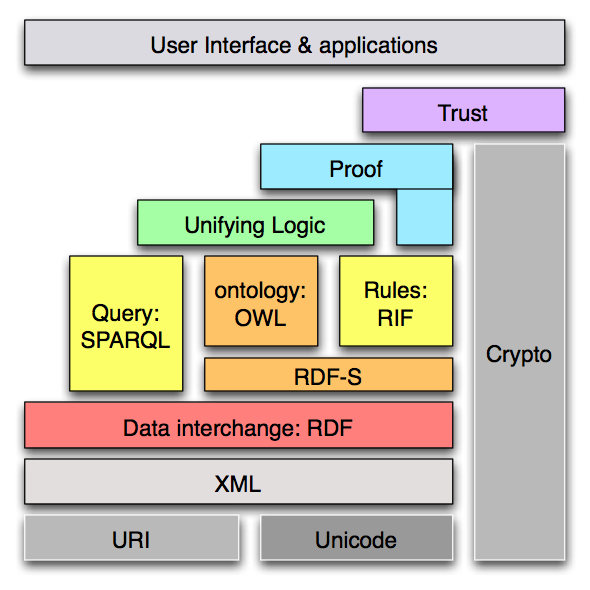
\includegraphics[width=0.65\textwidth]{figures/semantic_web.png}
\caption{The Semantic Web technologies}
\label{fig1}
\end{figure}

The RDF is widely used for representing KGs and this is the fundamental format for many KGs such as YAGO~\cite{ref28}, Freebase~\footnote{\url{https://developers.google.com/freebase/}}, Wikidata\footnote{\url{https://www.wikidata.org}}, etc. Several prominent examples of KGs and their sizes are reported in Table~\ref{table1}~\cite{ref27}. Google's Knowledge Graph is the largest among all the KGs mentioned in the table with 18 billions facts.

Though having different number of predicates, entities and facts, these graphs share the following common properties~\cite{ref27}:

\begin{itemize}
\item KGs reflect facts about the real world.
\item KGs cover different domains, for example, YAGO is a general purpose KG while IMDB focuses on the movie domain.
\end{itemize}

\begin{table}
\begin{center}
\begin{tabular}{|c|c|c|c|c|}
\hline
Name & Instances & Facts & Types & Relations\\
\hline\hline
DBpedia (English) & 4,806,150 & 176,043,129 & 735 & 2,813\\
\hline
YAGO & 4,595,906 & 25,946,870 & 488,469 & 77\\
\hline
Freebase & 49,947,845 & 3,041,722,635 & 26,507 & 37,781\\
\hline
Wikidata & 15,602,060 & 65,993,797 & 23,157 & 1,673\\
\hline
NELL & 2,006,896 & 432,845 & 285 & 425\\
\hline
OpenCyc & 118,499 & 2,413,894 & 45,153 & 18,526\\
\hline
Google's Knowledge Graph & 570,000,000 & 18,000,000,000 & 1,500 & 35,000\\
\hline
Google's Knowledge Vault & 45,000,000 & 271,000,000 & 1,100 & 4,469\\
\hline
Yahoo! Knowledge Graph & 3,443,743 & 1,391,054,990 & 250 & 800\\
\hline
IMDB & 117,551 & 134,639 & 17,049 & 39 \\
\hline
\end{tabular}
\end{center}
\caption{List of typical knowledge graphs}
\label{table1}
\end{table}

\section{Statistics-based Approaches for Relational Learning}

Relational Learning is a research field that focuses on ``representing, reasoning and learning in domains with complex relational structure"~\cite{ref43}. Many frameworks in this field can be fruitfully applied in the Semantic Web context. In this section, we discuss Relational Learning from statistics point of view. The statistics-based approaches focus on building models with latent features which are not directly observable from the original data~\cite{ref1}. The core idea is to infer correlation between objects based on selected hidden features.

RESCAL is one of the principal algorithms in this direction where relations of all hidden feature pairs are taken into consideration to measure likelihood of true facts~\cite{ref2, ref3}. This method is extended to classical tensor decomposition algorithm~\cite{ref4} and neural tensor network~\cite{ref5}.

While many tensor factorization methods use subject, predicate and object as three dimensions to model a KG as a cube, some algorithms transform this cube into two dimensional data in a preprocessing step. For instance, in~\cite{ref6, ref7} subject and object in every triple are merged into a single element representing a pair of entities.% A similar preprocessing step which we call data flattening is discussed in Section~\ref{system:discuss} in more details.

Distance-based models use the intuition that entities have high chance to be related to each other if their hidden representation features are close to each other. The closeness can be checked based on some predefined distance measures. This approach is expanded to structure embedding models in~\cite{ref8}.

\section{Logic-based Approaches for Relational Learning}

The logic-based approaches aim at finding observable patterns in order to infer new links in the KG~\cite{ref1}. Since the patterns can be directly seen in the data, these algorithms are more interpretable than the ones based on statistical approaches. For instance, a pattern extracted from the graph in Figure~\ref{fig1.1} can be represented as rule~\ref{rule1} ($\mi{r1}$). This rule reflects a triangular pattern in the KG, and since the rules are extracted from the graph, the predicates correspond to the edge labels. Since this pattern is frequently observed, it can be extracted to predict new links in the KG. For instance, if we apply the rule $\mi{r1}$ to the KG in Figure~\ref{fig1.1}, we can deduce the facts \textit{livesIn(Lucy, Amsterdam)} and \textit{livesIn(Dave, Chicago)}.

In the rest of this section, we review some of the most prominent logic-based relational learning systems in details and illustrate them with typical tools.

\subsection{Inductive Logic Programming Systems}

Inductive Logic Programming~\cite{ref9} (ILP) is a combination of Machine Learning and Logic Programming fields whose goal is to generate hypothesis from background knowledge and specific examples, which are normally classified into positive and negative ones. The aim is to find a hypothesis that covers all positive examples and none of the negative ones.

Rule mining is a core problem in ILP, however, applying ILP algorithms to Semantic Web data is problematic for the following reasons. First, ILP tools are not scalable for large knowlege graphs such as YAGO, Freebase, Wikidata~\cite{ref10}. In some experiments conducted in~\cite{ref10}, it has been shown that the cutting edge ILP tools, for example, ALEPH~\cite{ref14, ref10}, QuickFoil~\cite{ref15, ref10} require several days to process the YAGO KG.

Second, ILP methods use closed world assumption (CWA), under which a given KG is assumed to be complete and missing facts are treated as false rather than unknown. ILP methods require both positive and negative examples like traditional machine learning algorithms. One cannot rely on CWA in our problem since in the KGs the positive examples are incomplete and negative ones are unknown~\cite{ref10}.

Third, most ILP algorithms generate Horn rules without exceptions~\cite{ref11}. These rules often have low precision. One of the possible ways to improve the quality of the facts the rules predict is to add their appropriate exceptions. Therefore, mining exceptions for rules is an important task which we study in this work. In the following paragraphs, some popular ILP systems are described in details.

\textbf{ALEPH.} This name stands for A Learning Engine for Proposing Hypotheses which is one of the typical systems in ILP. The tool is developed and extended from P-Progol~\footnote{\url{http://www.cs.ox.ac.uk/activities/machinelearning/Aleph/aleph}}. Like many other ILP systems, as input ALEPH receives the background knowledge and sets of positive and negative examples. After that, it generates a set of rules as a hypothesis set. More specifically, the tool processes data in the following steps:

\begin{itemize}
\item ALEPH picks an example to hypothesize and terminates if no such example is found.
\item Then the most specific rule that infers the example is computed.
\item Among all subsets, i.e., combinations of atoms in the most specific rule, the one with the highest score is added to the hypothesis set.
\item All examples inferred by the chosen hypothesis are removed from the data and the process starts again from the first step.
\end{itemize}

Though this algorithm is among the most popular ones in ILP, experiments in~\cite{ref10} show that its runtime is extremely slow. This demonstrates the unsuitability of ALEPH for large datasets.

\textbf{QuickFOIL.} To address the scalability issues of ILP systems, an optimized version of FOIL~\cite{ref36}, i.e., the system QuickFOIL~\cite{ref45} has been developed, which performs the following steps:

\begin{itemize}
\item First, QuickFOIL produces a new Horn rule that maximizes the difference between the number of covered positive and negative examples in the training data. This criteria is different from traditional ILP where among the rules that do not infer negative examples, the one covering the highest number of positive examples is chosen.
\item Second, whenever the chosen rule covers an example, the latter is removed from the set of positive ones~\cite{ref10}. Intuitively, the collection of found rules at each step can be used to summarize original dataset. QuickFOIL uses pruning techniques where duplicates (i.e., rules that are equivalent to those generated before) are removed to process large-scale input with millions of facts.

\end{itemize}

\subsection{Relational Learning Systems}

Relational Learning systems do not require negative examples in the data, and they also work well under the Open World Assumption (OWA). This makes them attractive for our setting. In the following paragraphs, some Relational Learning tools are described in details.

%In addition, with the aim to expand KG, new facts generated by applying rules as an output of Relational Learning to the original KG are more precise than those of traditional Information Extraction~\cite{ref29}. Indeed, relational learning methods have been successfully applied to predict facts in YAGO2~\cite{ref30}.
\textbf{WARMR.} The WARMR~\cite{ref16, ref17} system represents a combination of traditional ILP and Relational Learning approaches. It extends APRIORI algorithm~\cite{ref44} to the relational setting and exploits a pruning technique in level-wise search to mine patterns. More specifically, at each level, infrequent queries are removed and the remaining frequent ones are expanded using the above operation. New queries are deleted if they can be expanded from an infrequent pattern in the previous level. This step is repeated until we cannot generate new queries. To check the runtime performance of WARMR, the authors of AMIE+~\cite{ref10} test it on the YAGO dataset. The tool processes more than a day with YAGO2. WARMR is developed with ProLog, which not particularly scalable for large datasets~\cite{ref10}.

\textbf{AMIE(+).} The scalability issues as well as CWA assumption issues of ILP are tackled in the AMIE(+)~\cite{ref10} system. This tool receives a large KG as input and generates top positive Horn rules ranked based on a certain association rule score. Initially, AMIE begins with a list of rules with empty body and a binary head predicate. After that, the rules are expanded with additional relations and variables using three mining operators. These operators are executed by query manipulation to explore new predicates and instances. As regards the implementation, AMIE uses in-memory database with fact indexes to run select and existence queries.

AMIE+ is an optimized version of AMIE. The authors introduce three main pruning strategies: maximum length constraint, quality condition and simplifying query. More specifically, in the first strategy, a rule is not expanded if its length reaches a threshold. In the second strategy, if confidence of a rule is already 100\%, the rule cannot be better and does not need to be extended. In the final strategy, approximation techniques are applied to assess the confidence of a given rule. Experimental work in~\cite{ref10} shows that this platform can process millions of triples in RDF graph and it surpasses other methods in terms of the run time.

\textbf{RDF2Rules.} The RDF2Rules~\cite{ref29} focuses on mining cyclic patterns from KGs, which are postprocessed and cast into rules. This tool improves rule quality by inserting entity types to their bodies, for example, \textit{diedIn(X,Y) $\leftarrow$ wasBornIn(X,Y), people(X), country(Y)} is expected to be more accurate than \textit{diedIn(X,Y) $\leftarrow$ wasBornIn(X,Y)}. Furthermore, they introduce a new confidence measure that exploits types of entities to verify rule quality. Experiments show that this tool is effective, especially with rules containing entity types, and it often outperforms AMIE+. However, the form of the mined rule is restricted to cycles, which makes the system more restrictive than the AMIE+ system.

Like other ILP platforms, Relational Learning tools only focus on positive (Horn) rules and they do not learn nonmonotonic rules, i.e., rules with exceptions. In this work, we aim at bridging this gap and develop method to learn the latter types of rules.

\subsection{Nonmonotonic Rule Mining Systems}
\label{related-work-nonmonotonic-rule-mining-systems}

Rules with exceptions are traditionally learned by nonmonotonic rule learning systems. The research work in~\cite{ref32} is devoted to the problem of learning nonmonotonic rules. The idea behind it is to convert an ILP task into an ALP~\cite{ref31} instance, and then, the way the ALP instance is solved can be mapped to the ILP one 's solutions. However, this system adopts CWA, and therefore cannot be applied in our work. There is another nonmonotonic rule learning method that accounts for incomplete data~\cite{ref34} where a coordination of Semantic Web ontology and positive/negative rules is exploited to explore patterns. The work~\cite{ref34} pays attention to complicated communication between different reasoning components. This is different from the current work where we focus on the quality of the predicted data.

\textbf{Nonmonotonic Rule Mining under OWA over the flattened data.} The work~\cite{ref12} made some steps towards learning nonmonotonic programs from incomplete KGs. However, the developed methods work only on flattened KGs, i.e., the graphs in which all RDF triples are converted to unary facts by concatenating predicates and objects. More specifically, a binary fact such as \textit{bornIn(s1, US)} is transformed to a fact in the unary form \textit{bornInUS(s1)}. This way, a KG is converted to a binary transaction table (for example, see Table~\ref{table2}) where 1 (respectively, 0) appears in the intersection of a column $c$ and a row $r$ if the fact $c(r)$ is present (respectively, not present) in the KG. For instance, Table~\ref{table2} reflects that \textit{bornInUS(s1)} is included in the KG while \textit{livesInUS(s6)} is not. This representation allows one to apply highly optimized Item Set Mining algorithms~\cite{ref37} to extract data patterns which can then be used to create positive association rules~\cite{ref13}.

\begin{table}
\begin{center}
\begin{tabular}{|c|c|c|c|c|}
\hline
 & bornInUS & livesInUS & immigratesToUS & livesInUK\\
\hline\hline
s1 & 1 & 1 & 0 & 0\\
\hline
s2 & 1 & 0 & 1 & 1\\
\hline
s3 & 1 & 1 & 0 & 1\\
\hline
s4 & 0 & 0 & 1 & 0\\
\hline
s5 & 1 & 0 & 0 & 1\\
\hline
s6 & 0 & 0 & 1 & 1\\
\hline
s7 & 0 & 0 & 1 & 1\\
\hline
s8 & 1 & 0 & 0 & 0\\
\hline
s9 & 1 & 1 & 1 & 1\\
\hline
s10 & 0 & 1 & 0 & 1\\
\hline
\end{tabular}
\end{center}
\caption{Transaction table as flattened knowledge graph data.}
\label{table2}
\end{table}

In the next step, the exceptions for each rule are found and ranked based on several score measures and innovative concept of Partial Materialization (PM)~\cite{ref12}. The idea behind this is to enable the interaction between the rules. A difference between this thesis and~\cite{ref12} stems from the format of the data. While in~\cite{ref12} binary facts are translated into unary ones, in this thesis we keep the facts in their natural relational format.

\section{Text-based Approaches for Relational Learning}

Both statistics-based and logic-based approaches are internal methods, i.e., only data inside the graph is used to infer new relations. We now discuss other approaches that require data outside the KG, i.e., web pages linking to objects or big collection of documents.

Wikipedia pages can be used to identify relations between entities~\cite{ref18}. On a larger scale, an algorithm in~\cite{ref19} is developed to learn lexical predicate patterns, for example, \textit{isMarriedTo} predicate in Figure~\ref{fig1.1} can be expressed  as ``married to", ``engaged with", etc in some documents. Then these patterns are being searched for all over the Internet to find subject-object pairs corresponding to them. These new pairs can be added to the original graph. For example, in ~\cite{ref19} a  big text corpus is used to learn relations.

In~\cite{ref20} the authors refine KGs by exploiting the assumption that entities appearing in the same table should have the same relations. Similarly, ~\cite{ref21} and ~\cite{ref22} exploit page lists and HTML tables, respectively.

Instead of documents, interlinks between the same entities in different KGs can be used to add new facts~\cite{ref23, ref24}. More specifically, relations of two entities in Freebase can be inserted into YAGO if they also appear in the latter KG. In~\cite{ref25} this approach has been extended to a probabilistic setting, where for every deduced relation a corresponding probabilistic weight is computed.